% !TeX spellcheck = en_US
\documentclass[a4paper]{scrartcl}

\usepackage[utf8]{inputenc}
\usepackage[english]{babel}
\usepackage[T1]{fontenc}
\usepackage{lmodern}
\usepackage{amsmath}
\usepackage{amssymb}
\usepackage{pdflscape}
\usepackage{geometry}
\usepackage{xcolor}
\usepackage{graphicx}
\usepackage{siunitx}
\usepackage{todonotes}
%\setlength{\parindent}{0pt}

\usepackage{biblatex}
\addbibresource{references.bib}


\geometry{a4paper, top=25mm, left=30mm, right=20mm, bottom=30mm,
headsep=10mm, footskip=12mm}

\newcommand{\itab}[1]{\hspace{0em}\rlap{#1}}
\newcommand{\tab}[1]{\hspace{.2\textwidth}\rlap{#1}}
\newcommand{\N}{\mathbb{N}}
\newcommand{\es}{\emptyset}

\title{Seminar on Algorithms for Compressed Graphs \\ Succinct Representation of Labeled Graphs}
\author{Matthias Dürksen}
\date{\today}
 

\begin{document}
\maketitle

\begin{abstract}
	Due to the increasing size of graphs and the associated memory requirements, the topic of graph compression is becoming more and more important. In this paper a coding for planar graphs is presented. These are converted into triangulated graphs and the set of edges is divided into three subsets so that each set is a tree. These are converted into parentheses and then combined. It is possible to store all information extremely compacted.
\end{abstract}


\section{Introduction}\label{sec:introduction}
This article describes the paper "Succinct Representation of Labeled Graphs"~\cite{SuccinctRepresentation} by Jérémy Barbay. This is a compression process for triangulated graphs. Graphs are an important data structures for computer science and are mainly used for linking elements.


\subsection{Motivation}


There are many applications where data is stored in the form of data and fast requests have to be possible. In this case an efficient storage is crucial to make this possible. In this approach we consider planar graphs as a subclass of graphs. Planar graphs are graphs that can be displayed on a two-dimensional surface in such a way that none of the edges overlaps with another edge. A use case here is the simplified road network. If there were no bridges or tunnels, the road system could be represented as a planar graph, where each intersection is a node and the roads are the edges. In order to be able to save this use case efficiently, we present here the approach of Jérémy Barbay~\cite{SuccinctRepresentation}.






\section{Succinct Representation}
The goal is to encode a graph as efficiently as possible and to be able to process query requests as efficiently as possible~\cite{SuccinctRepresentation}. Therefore triangulated planar graphs are converted into three trees, which in turn are converted into parenthesis. The parenthesis for the three trees are then converted to a nested parenthesis. This bracketed representation is the efficient coding where requests can be answered efficiently.





\subsection{Graph Model}
A graph $G=(V,E)$ consists of a set of nodes $V$ and a set of edges $E$. We consider undirected graphs so that the set of edges $E$ is undirected.
The succinct representation is constructed so that the coding only works for a subset of graphs, the undirected planar graph. A planar graph is a  graph$G$ that can represent nodes in a two dimensional plane so that no edges intersect with another edge. For an example of a planar graph, see Figure~\ref{fig:planar}.


\begin{figure}[h]
	\centering
	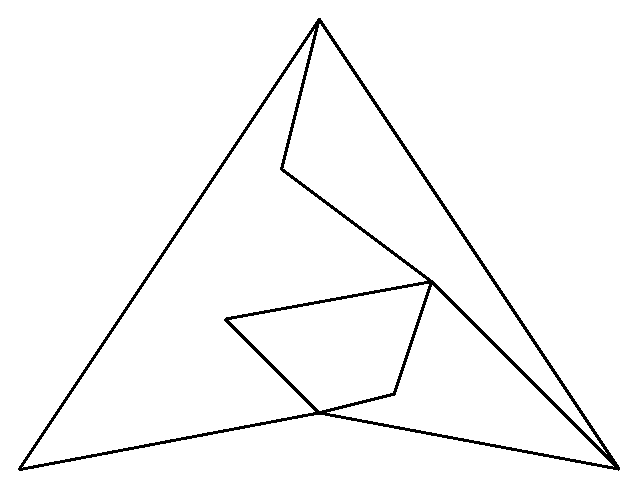
\includegraphics[width=0.4\textwidth]{img/planar}
	\caption{A planar graph}
	\label{fig:planar}
\end{figure}


In the first step, the planar graphs are converted to a triangulated planar graph. Each inner surface is supplemented by additional edges so that the surface becomes triangles. In this way, the entire graph can be transformed into triangular surfaces. 


The graph from Figure~\ref{fig:planar} becomes a triangulated planar graph by the graph, see Figure~\ref{fig:triangulated}.
Therefore it can be assumed that the graph always has three vertices which are adjacent to each other.


For our coding, the triangulated graph must also have exactly three nodes on the convex hull. This can be created by adding the three new nodes and placing them in three corners so far out that edges between the new nodes lie outside the old nodes and edges. These nodes will be connected in pairs and added to the previous graph. During triangulation, the newly instantiated surfaces will also be triangulated.
 These edges form the convex hull of the graph, where we call the three nodes $v_0,v_1$ and $v_{n-1}$.



\begin{figure}[h]
	\centering
	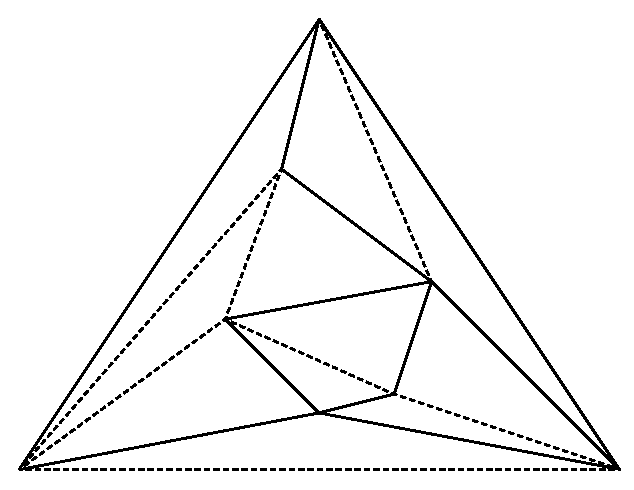
\includegraphics[width=0.4\textwidth]{img/triangulated}
	\caption{The triangulated  graph from Figure~\ref{fig:triangulated}}
	\label{fig:triangulated}
\end{figure}

\subsection{Schnyder realizer}
The graph is divided into three trees for further compression. For this a Schnyder realizer~\cite{schnyder} is used. This divides the graph into three trees $T_0,T_1,T_2$. Each inner edge is assigned to one of the three trees. These are assigned so that each inner node has three outgoing edges, where each outgoing edge contains to a different tree. In addition, the node can have incoming edges, where these must be arranged in a certain way. In Figure~\ref{fig:schnyderRealizer} we see the arrangement. The edges are arranged according to the pattern outgoing $T_0$, incoming $T_1$, outgoing $T_2$, incoming $T_0$, outgoing $T_1$, incoming $T_2$. The trees $T_0,T_1,T_2$ have as root the node $v_0,v_1,v_{n-1}$.


\begin{figure}[h]
	\centering
	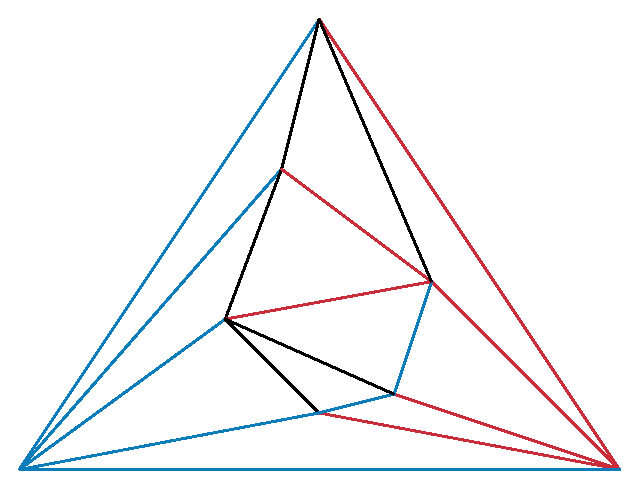
\includegraphics[width=0.6\textwidth]{img/exampleSchnyder}
	\caption{The trees in the graph which are formed on the basis of the Schnyder realizer}
	\label{fig:exampleSchnyder}
\end{figure}


\subsection{Traversal Orders}
The graph is divided into three subtrees using a Schnyder realizer, but the edges lying on the convex hull of the graph are not yet contained in the trees. In addition we have to number the nodes for the following brackets.
The two edges $(v_1,v_0),(v_{n-1},v_0)$, which lie on the convex hull, are assigned to the tree $T_0$ and the edge $(v_{n-1},v_1)$ is assigned to the tree $T_1$. So $T_0$ is an canonical spanning tree.

To number the nodes in $T_0$ a depth search in the node $v_0$ is executed counterclockwise and the visited nodes are ascending ordered, see Figure~\ref{fig:exampleTraversal}.

\begin{figure}[h]
	\centering
	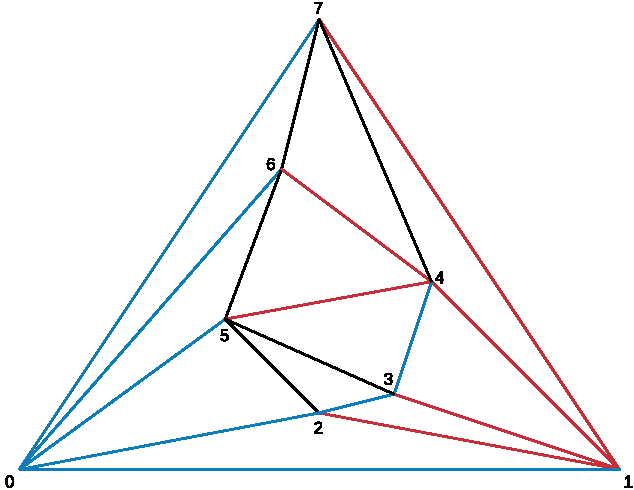
\includegraphics[width=0.6\textwidth]{img/exampleTraversal}
	\caption{The partitioned graph with the numbering by $T_0$}
	\label{fig:exampleTraversal}
\end{figure}




\subsection{Parenthesis}
The aim is to combine the trees with the help of brackets to a common brackets representation. To do this, we first generate the parenthesis for the individual trees and then combine them. For each of the trees $T_0,T_1,T_2$ the parenthesis is generated differently. We designate a pair of parenthesis as an opening parenthesis followed by a closing parenthesis.

Let's first look at the parenthesis for the tree $T_0$. Starting from the root $v_0$ this parenthesis is created. To encode the root we use pairs of brackets. For each of the children of depth 1 we create another pair of brackets in the pair of brackets. If a child $a$ of depth 1 has children of its own, its children are displayed as a pair of parenthesis in the pair of parenthesis for the node $a$. The children are included in the parenthesis on a level countering the clockwise direction. Thus the following recursive definition follows:

For all nodes $v$ of depth i applies:



\begin{equation}
\begin{split}
 i & =0 \rightarrow \text{pair of parenthesis}\\
i & >0 \rightarrow \text{insert pair of parenthesis in } parent(v)
\end{split}
\end{equation}

Figure~\ref{fig:parenthesisOne} shows how such a parenthesis for the tree $T_0$ looks like with our example.


\begin{figure}[h]
	\centering
	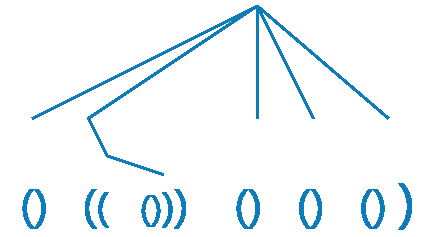
\includegraphics[width=0.7\textwidth]{img/parenthesisOne}
	\caption{The parenthesis of the  tree $T_0$}
	\label{fig:parenthesisOne}
\end{figure}





For the tree $T_1$ the parenthesis representation is generated differently. A pair of parenthesis is created for each child of the root $v_1$, but the pairs of parenthesis are not written one after the other on the same level, but nested together. Here the edges are passed counterclockwise again, so that the child $a$, which is visited first, is on the outside and the other children are written into the brace pair of $a$. If a node has $v$ children, the children are also nested into each other and packed in the place of the parenthesis, which comes directly after the closing parenthesis of $a$. The parenthesis for the tree $T_1$ from our example is shown in Figure~\ref{fig:parenthesisTwo}.


\begin{figure}[h]
	\centering
	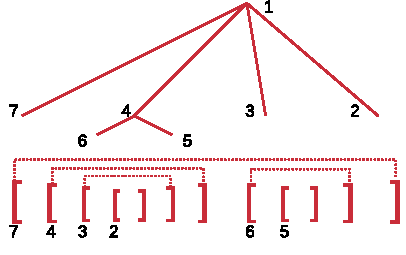
\includegraphics[width=0.7\textwidth]{img/parenthesisTwo}
	\caption{The parenthesis of the  tree $T_1$}
	\label{fig:parenthesisTwo}
\end{figure}


The parenthesis for the tree $T_2$ is created similar to the parenthesis for $T_1$. The children are nested again, but the children are passed clockwise. If a node $v$ has  children, these nested children are now written in front of the opening parenthesis of $v$. This procedure is illustrated by the example in Figure~\ref{fig:parenthesisThree}.


\begin{figure}[h]
	\centering
	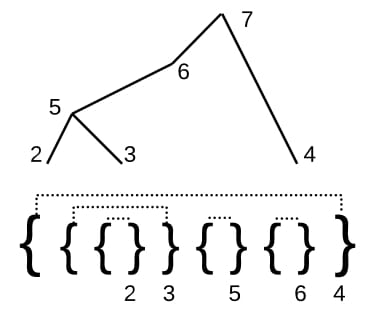
\includegraphics[width=0.7\textwidth]{img/parenthesisThree}
	\caption{The parenthesis of the  tree $T_2$}
	\label{fig:parenthesisThree}
\end{figure}

The three parenthesis must now be combined so that no information about the graph is lost. The parenthesis of a tree $T_i$ is called $S_i$. In order to be able to distinguish the parts of the different parenthesis according to the combination, we use different parenthesis symbols for each parenthesis. The parenthesis $S_0$ serves as the basic structure. The other two parenthesis are included in this. The parenthesis are created as follows.

\begin{itemize}
	\item $\forall e=(v_i,v_j)\in T_1: \text{ insert } '[' \text{ before } parenthesis(v_i)\in S_0 \text{ closed.}$
	\item $\forall e=(v_i,v_j)\in T_1: \text{ insert } ']' \text{ after } parenthesis(v_i)\in S_0 \text{ opened.}$
	\item $\forall e=(v_i,v_j)\in T_2: \text{ insert } ']' \text{ after } parenthesis(v_i)\in S_0 \text{ opened.}$
	\item $\forall e=(v_i,v_j)\in T_2: \text{ insert } '[' \text{ before } parenthesis(v_i)\in S_0 \text{ closed.}$
\end{itemize}
In the example, the three parenthesis become the combined representation in Figure~\ref{fig:parenthesisCombi}.
This creates a parenthesis that contains three types of parenthesis, each parenthesis still being a valid parenthesis.

\begin{figure}[h]
	\centering
	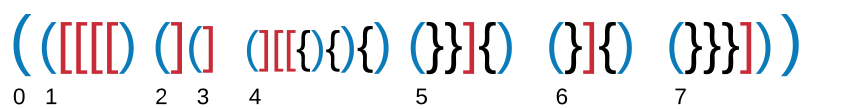
\includegraphics[width=0.8\textwidth]{img/parenthesisCombi}
	\caption{The parenthesis of the merges trees}
	\label{fig:parenthesisCombi}
\end{figure}

\subsection{Query}
The coded data structure also supports efficient queries. An overhead of $o(m)$ bits was accepted to implement some queries without sacrificing performance. Among the supported queries are the adjacency query of a node as well as on the degree of a node. These and other queries are supported with $O(1)$ time requirements. 

\subsection{Size complexity}
The parenthesis representation consists of three different types of parenthesis, whereby 2 symbols are required for each type (opening and closing parenthesis). This means that a total of 6 different characters are required. Each edge of the graph is coded exactly once and one opening and one closing bracket are required per edge. Nodes do not have to be encoded separately, since the information indirectly contains the edges. Thus $2m$ symbols are needed for the representation, at m the number of edges is in G. Since we need a total of 6 different symbols, three times each the opening and closing parenthesis, $\lceil log_2 6\rceil=3$ bits are sufficient. In total we need $2m\lceil log_2 6\rceil+o(m)$ bits, where $o(m)$ is an overhead to make the queries more efficient. 


\section{Conclusion \& Future Work}
In this paper we have presented an approach to efficiently store planar graphs and still enable efficient queries. Therefore the planar graph is converted into a triangulated graph. This graph is then divided into three trees using the Schynder realizer. These can then be converted to parentheses with a special construction, which is then combined to form a complete parenthesis. From this all information of the graph can be retrieved and for many queries even lost without performance.


Furthermore, it should be investigated which practical examples of planar graphs exist in the economy where coding could be used. Furthermore, the paper reports about an extension to k-Page graphs and should be investigated, which graphs can be converted to k-Page graphs and if this can increase the number of applications significantly.

\pagebreak


\printbibliography







\end{document}